\documentclass[10pt]{article}

\usepackage{fullpage} % Package to use full page
\usepackage{parskip} % Package to tweak paragraph skipping
\usepackage{tikz} % Package for drawing
\usepackage{amsmath}
\usepackage{hyperref}
\usepackage{graphics,multirow,cases,algorithm,algpseudocode}
\usepackage{booktabs,color,comment}
\usepackage[english]{babel}
\usepackage{amsmath,amsthm,amssymb,verbatim,bbm}
%\usepackage[framed,numbered,autolinebreaks,useliterate]{mcode}
\usepackage{url}
\usepackage{nomencl}
\usepackage{enumitem}
\usepackage{siunitx}
\usepackage{float}

\usepackage[normalem]{ulem}

\newcommand*{\bbar}[1]{\bar{\bar{#1}}}

\newcommand{\R}{{\mathcal{R}}}
\newcommand{\T}{{\mathcal{T}}}
\newcommand{\D}{{\mathcal{D}}}
\newcommand{\F}{{\mathcal{F}}}
\renewcommand{\S}{{\mathcal{S}}}
\newcommand{\spb}{{\smallskip}}
\newcommand{\mpb}{{\medskip}}
\newcommand{\bpb}{{\bigskip}}
\newcommand{\IN}{{\mathbb{N}}}
\newcommand{\IM}{{\mathbb{M}}}
\newcommand{\IZ}{{\mathbb{Z}}}
\newcommand{\IR}{{\mathbb{R}}}
\newcommand{\IE}{{\mathbb{E}}}
\newcommand{\IP}{{\mathbb{P}}}
\newcommand{\IC}{{\mathbb{C}}}
\newcommand{\mO}{{\mathcal{O}}}
%\newcommand{\IR}{{\mathbb{R}}}
%\newcommand{\IC}{{\mathbb{C}}}
%\newcommand{\IN}{{\mathbb{N}}}
%\newcommand{\IE}{{\mathbb{E}}}
%\newcommand{\IP}{{\mathbb{P}}}
\newcommand{\mF}{{\mathcal{F}}}
\newcommand{\mE}{{\mathcal{E}}}
\newcommand{\tT}{\intercal}
\newcommand{\mT}{{\mathcal{T}}}
\newcommand{\mconv}{{\mathrm{conv}}}
\newcommand{\mC}{{\mathcal{C}}_{2 \pi}}
\newcommand{\IX}{{\mathbb{X}}} %domain
\newcommand{\IS}{{\mathbb{S}}} %domain
\newcommand{\ID}{{\mathbb{D}}}
\newcommand{\IY}{{\mathbb{Y}}}
\newcommand{\cSm}{{\cal S}^{(m)}}
\newcommand{\cS}{{\cal S}_N}
\newcommand{\SM}{{\mathcal{P}}}
\newcommand{\SN}{{\mathcal{Q}}}
\newcommand{\SB}{{\mathcal{B}}}
\newcommand{\SD}{{\mathcal{D}}}

\newcommand{\iin}{\frac{i}{n}}
\newcommand{\jjn}{\frac{j}{n}}
\newcommand{\sumi}{\dsum_{i=1}^{n}}
\newcommand{\sumN}{\dsum_{i=1}^{N}}
\newcommand{\sumT}{\dsum_{t=1}^{T}}
\newcommand{\sumj}{\dsum_{j=1}^{n}}
\newcommand{\sumij}{\dsum_{i<j}}
\newcommand{\Xt}{{X_{t}}}
\newcommand{\Yt}{{Y_{t}}}
\newcommand{\la}{{\lambda}}
\newcommand{\bA}{{\bf A}}
\newcommand{\bB}{{\bf B}}
\newcommand{\bC}{{\bf C}}
\newcommand{\bAs}{{\bf A}_{\epsilon}}
\newcommand{\Bs}{B^{(\epsilon)}}
\newcommand{\bT}{{\bf T}}
\newcommand{\bu}{{\bf u}}
\newcommand{\bb}{{\bf b}}
\newcommand{\cT}{{\cal T}}
\newcommand{\cW}{{\cal W}}
\newcommand{\cC}{{\cal C}_{\epsilon}}
\newcommand{\cD}{{\mathcal{D}}}
\newcommand{\dx}{\Delta x}
\newcommand{\dt}{\Delta t}
\newcommand{\ep}{\epsilon}
\newcommand{\pC}{\partial C}

\makenomenclature
\renewcommand{\nomname}{List of Symbols}
%\renewcommand{\nompreamble}{The next list describes several symbols that will be later used within the body of the document}

\newenvironment{definition}[2][Definition]{\begin{trivlist}
\item[\hskip \labelsep {\bfseries #1}\hskip \labelsep {\bfseries #2.}]}{\end{trivlist}}
\newenvironment{theorem}[2][Theorem]{\begin{trivlist}
\item[\hskip \labelsep {\bfseries #1}\hskip \labelsep {\bfseries #2.}]}{\end{trivlist}}
\newenvironment{lemma}[2][Lemma]{\begin{trivlist}
\item[\hskip \labelsep {\bfseries #1}\hskip \labelsep {\bfseries #2.}]}{\end{trivlist}}
\newenvironment{exercise}[2][Exercise]{\begin{trivlist}
\item[\hskip \labelsep {\bfseries #1}\hskip \labelsep {\bfseries #2.}]}{\end{trivlist}}
\newenvironment{reflection}[2][Reflection]{\begin{trivlist}
\item[\hskip \labelsep {\bfseries #1}\hskip \labelsep {\bfseries #2.}]}{\end{trivlist}}
\newenvironment{proposition}[2][Proposition]{\begin{trivlist}
\item[\hskip \labelsep {\bfseries #1}\hskip \labelsep {\bfseries #2.}]}{\end{trivlist}}
\newenvironment{corollary}[2][Corollary]{\begin{trivlist}
\item[\hskip \labelsep {\bfseries #1}\hskip \labelsep {\bfseries #2.}]}{\end{trivlist}}

\DeclareMathOperator*{\argminA}{arg\,min} % Jan Hlavacek
\DeclareMathOperator*{\argminB}{argmin}   % Jan Hlavacek
\DeclareMathOperator*{\argminC}{\arg\min}   % rbp


% Latin text highlight
\def\latin#1{\emph{#1}}

% Mark-up commands
\def\Red#1{\textbf{\textcolor{red}{#1}}}	% for authors
\def\Blue#1{\textbf{\textcolor{blue}{#1}}}	% for reviewers


\title{TDA - filament network classification}
%\author{Le Yin, Ephy Love}
\date{November 2019}

% path to graphics
\graphicspath{{figures/}}

\begin{document}

\maketitle

\begin{abstract}

The actin cytoskeleton plays a critical role in plant cells. The filamentous structure of actin proteins can be viewed as a network endowed with a topology. We classify myosin-mutant from wildtype \textit{Arabidopsis} root cells by their actin network topologies, captured in confocal microscopy images. We benchmark our classifier against several distance and non-distance based classifiers, using a simulated dataset to compare sensitivities. We succeed in classifying the simulated networks with very high accuracy and carry over the highest accuracy method to classify the \textit{Arabidopsis} root cell images. Our top performing method is an automated classifier, combining topological data analysis (TDA) with a machine learning framework in order to investigate and leverage the topology of actin networks. Our classifier is non-distance-based, instead using a persistence vectorization. We attain additional power, at a low computational cost, through sub-sampling.

    %\textbf{Keywords:} 
    
    %\textbf{Running head:} 
\end{abstract}

\section{Introduction}
The actin cytoskeleton is a complex network of proteins that is present in all eukaryotic cells. In addition to its function as cellular scaffolding, the actin cytoskeleton enables several basic cellular functions including the control of cellular shape and direction of movement \cite{thomas2009actin}. These basic functions are critical to many higher order physiological processes such as cell division, expansion, mobility and motility\cite{freedman2017versatile}. 

Actin filament organization is thought to be largely governed by the interaction of the filaments themselves and by myosin motor proteins. Actin filaments are polar structures, ploymerized by globular actin proteins. Many actin-binding proteins have potential to bind to actin filaments at various sites along the filament. These binding proteins allow actin filaments to spatiotemporally assemble and disassemble. The binding proteins give rise to a dense cross-linking where filaments develop into networks consisting of many filaments and very many binding sites. Therefore, one key driver of actin network dynamics  is the relationship between actin-binding proteins, individual filaments, and emergent networks \cite{freedman2017versatile,freedman2018nonequilibrium}. Another key driver is the activitity of myosin motor proteins \cite{ueda2010myosin,madison2015class,peremyslov2010class,park2013myosin}, which perform several critical functions including pulling intracellular bodies about the cell. To understand certain behaviors of cells, it is of tremendous importance to understand the processes that govern actin filament network organization including the binding of actin filaments and the role of myosin motor activity.

Our goal is to develop a general framework for the classification of actin network topologies. The images of actin networks we examined are captured via confocal microscopy. These images are very high resolution (typically $1500\times400$ to $2500\times500$ pixels, where a pixel is approximately $\SI{.04}{\micro\metre}^2$), but suffer from several types of noise such as: filaments moving through the focal plain, rounding of the cell at the edges, neighboring cells poluting the image, and changes in microscopic conditions/settings. Consequently, confocal microsocopy data have the advantage of providing many high quality data at the expense of also including many noisy data. In order to automatically study these images, without myriad interjections by researchers (and thus eliminating a potential introduction of bias), an automated tool is called for which is highly robust to these types of noise. This work seeks to develop a classifier, robust to the noise of confocal microscopic images of actin networks, and requiring minimal intervention from researchers.

In the fast developing field of machine learning, topological data analysis (TDA) has become increasingly popular as a tool for noisy network and signal classification. To date, researchers have used TDA to solve many real-world problems including signal identification \cite{marchese2016topological}, materials classification \cite{hiraoka2016hierarchical,maroulas2019bayesian}, shape recognition \cite{bonis2016persistence,li2014persistence}, histologic image analysis \cite{belchi2018lung,nicolau2011topology,singh2014topological}, ecology of human mobility \cite{chen2017measuring,chen2019generalized}, and cosmology \cite{sousbie2011persistent,van2010alpha}. A review of TDA and its applications is provided in \cite{wasserman2018topological}. A sub-method of TDA, persistence homology, is a popular mechanism used to measure differences in topological features, due to its robustness in the face of purturbated data. Persistence homology records when homological features (connections and voids) appear and vanish in data. These patterns vary between data. All of the appearances and disappearances of homological features are summarised in persistence barcodes and/or diagrams. In this work, we encode the geometric features of filaments networks into persistence diagrams and show a method of classification on the vectorization of the persistence space (a persistence space is not itself a vector space, and, for instance, may not have a unique mean \cite{mileyko2011probability}). We compare this approach to traditional, distance-based classififications which attempt to summarize the similarities of the actin network topologies in the persistence space.

We are aided in our investigation of classification methods of actin networks by a dataset of simulated networks, which we use to benchmark our candidate methods. We are provided the outputs of simulations which combine theoretical physical properties with experimental stochastic simulations in order to emulate actin network dyanmics. These simulations allow the researcher to control the instantiating factors which will drive the emergent structure of the networks. Varying the initial conditions enables us to compare the conditional difference in outcomes of the simulated networks. This experimental strategy can provide an opportunity to independently examine the role individual factors play in the process of network formation. These factors could include the cross-linker density(number of cross-linkers per certain area), cross-linker stiffness, maximum angle that can exist between two filament segments to be crosslinked, and so on \cite{freedman2017versatile,freedman2018nonequilibrium}. This control mechanism also gives us the opportunity to test our classification methods on an analagous, highly controlled and clean dataset.

After testing several methods of actin network classification on the simulated data, we take our top performing method and adapt it to the classification of microscopy images. We test our classifier, by measuring it's accuracy in a task of supervised learning wherein we label  myosin-mutant (MM) and wildtype (WT) \textit{Arabidopsis} root cells. The MM cells have a genetic knockout on one myosin motor protein and the WT cells are a control with no knockout. Our top performing method provides very high accuracy in classifying the simulated data, but less so in the microscopy data. We address the likely reasons for this descrepency as well as future improvements in our final discussion.

The structure of this work is as follows: In Section \ref{sec:networksAndHomology}, we describe the data and introduce persistence homology. Section \ref{sec:methods} describes our methods including several detailed algorithms for classifying simulated and imaged filament networks. Section \ref{sec:results} compares the results from the simulated networks and exhibits teh final results on the classfication of microscopy images. Finally, in Section \ref{sec:discussion}, we discuss the implications, limitations and conclusions of our work.

\section{Filament Networks and Persistence Homology}\label{sec:networksAndHomology}
To quantify the differences in filament networks, we need to tranform our data in a manner that reveals its hidden geometric features. We perform this transformation using simplicial complexes in a manner typical of persistence homology. We use the 2-dimensional coordinates of sampled points along the filaments as initial nodes. Simplcial complexes provide a bridge between the data space and a topological space in which computation of distances between sets of data points can be realized. A simplicial complex is a finite collection of simplices of different dimensions such that faces of simplices are also simplices, and intersections of the simplices are either empty or a face of both \cite{edelsbrunner2010computational}. In particular, higher dimensional simplices are constructed from lower dimensional simplices. Vertices are 0-dim simplices. A 1-dim simplex is called an edge and is created by its two vertices as faces (note that a higher dimensional edge is constructed from lower dimensional points). A 2-dim simplex or a triangle has three edges as faces. Further more, a 3-dim simplex or a tetrahedron has four triangles as faces, another nesting of several lower dimensional features to build one of higher dimension.

\subsection{Data}
We are provided data in two spaces. The focus of this work is to develop a method for the classification of actin networks in confocal microscopic imagery. These data are given to us in the form of one 2-dimensional image per cell, where the data can be seen as a rectangular lattice of pixel instensities. We are also provided benchmarking data that come from simulations. The outputs we are provided from these simulations are point-clouds, with coordinates in 2-dimensions.

\textbf{Microscopy data:}
The microscopy data were provided in the form of one grayscale image per cell. An example image is shown in Figure \ref{fig:wtCell}. The actin filaments fluoresce in the images and so the intensity of each pixel of an image can be thought of as indicating the likely presense of a filament in that region of the cell. In order to study the homology of an actin network, we must perform a topological tranformation on the data. Since the images contain hundreds of thousands of pixels, we chose to sample from the images a set of points, where the probability of choosing a pixel is propotionate to the pixel's intensity. We make a choice of a number of pixels that we think is likely to sufficiently summarize a network. We sample the pixels coordinates, weighted by pixel intensity, to get a set of points in 2 dimensions. We can then perform our topological transformation on these new point clouds.

\begin{figure}[H]
	\begin{center}
		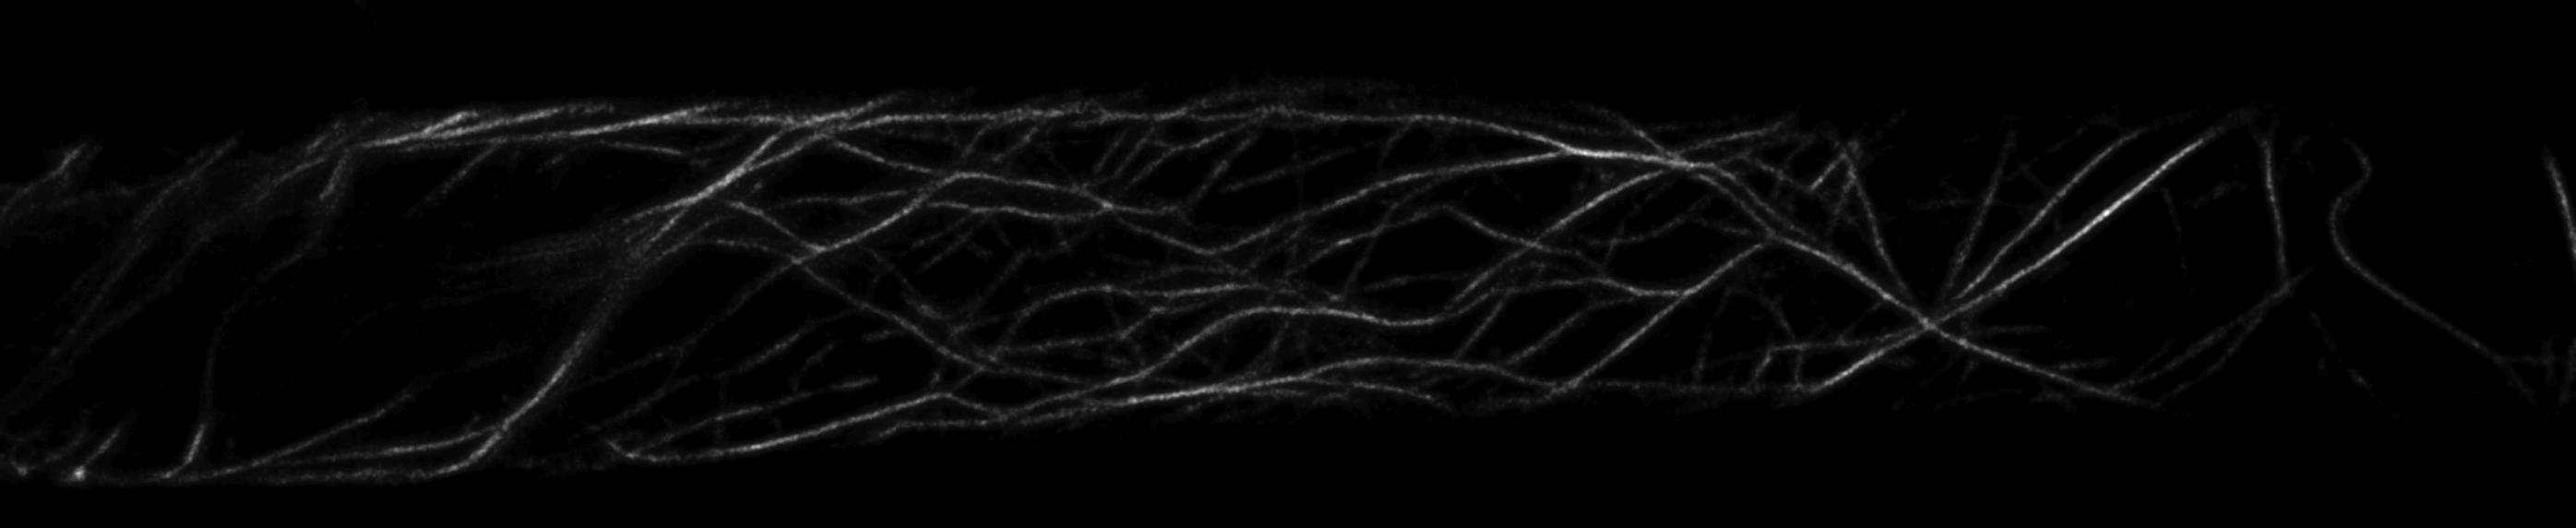
\includegraphics[width=1\textwidth]{figures/wtCell.png}
	\end{center}
	\caption{Example of an original, grayscale WT cell image.}
	\label{fig:wtCell}
\end{figure}

We are given labeled images of cells belonging to one of two classes: MM or WT. The MM cells have a genetic knockout such that they do not a produce one of their myosin proteins. The WT cells are the control with no knockout. Myosin motor proteins are known, via empirical observation, to influence the connectivity and shape of the actin filament network \cite{ueda2010myosin,madison2015class,peremyslov2010class,park2013myosin}. Therefore, we expect to the MM and WT cells to differ in their topologies.

\textbf{Simulated data:}
Our synthetic data come from simulations with varried numbers of crosslinking protiens. As discussed, actin filaments are thought to be organized by cross-linking on actin-binding proteins. Filaments and inter-filament structure can then be simulated by a physical model \cite{freedman2017versatile,freedman2018nonequilibrium}. The change of initial conditions in a eukaryotic cell will cause variation in later measurement of filament networks. Our network data are simulated with three different cross-linker densities. Higher cross-linker density means more opportunities for filaments to be cross-linked, i.e. the binding and unbinding processes can be more active. As shown in Figure \ref{fig:rawdata}(a), three kinds of filaments networks were simulated with different numbers of cross-linkers:  $825$, $1650$ and $3300$. All simulated cells were bound by a $\SI{20}{\micro\metre} \times \SI{20}{\micro\metre}$ square. Therefore, the cross-linker density of each network is $2.06$, $4.13$ and $8.25$ per $\SI{}{\micro\metre}^2$, respectively. In each network, there are a total of $100$ filaments with average length $\SI{10}{\micro\metre}$. In figure \ref{fig:rawdata}, the filaments are modeled as polar worm-like chains in red and blue dots represent barbed ends of these filaments. The locations of the actin beads that make up the filaments, which are shown as small black circles in Fig. \ref{fig:rawdata}(b) are the outputs that we are provided. Each actin bead is of radius $\SI{0.5}{\micro\metre}$. These actin beads will act as our point clouds in the topological transormations of these simulated data.

\begin{figure}[H]
	\begin{center}
		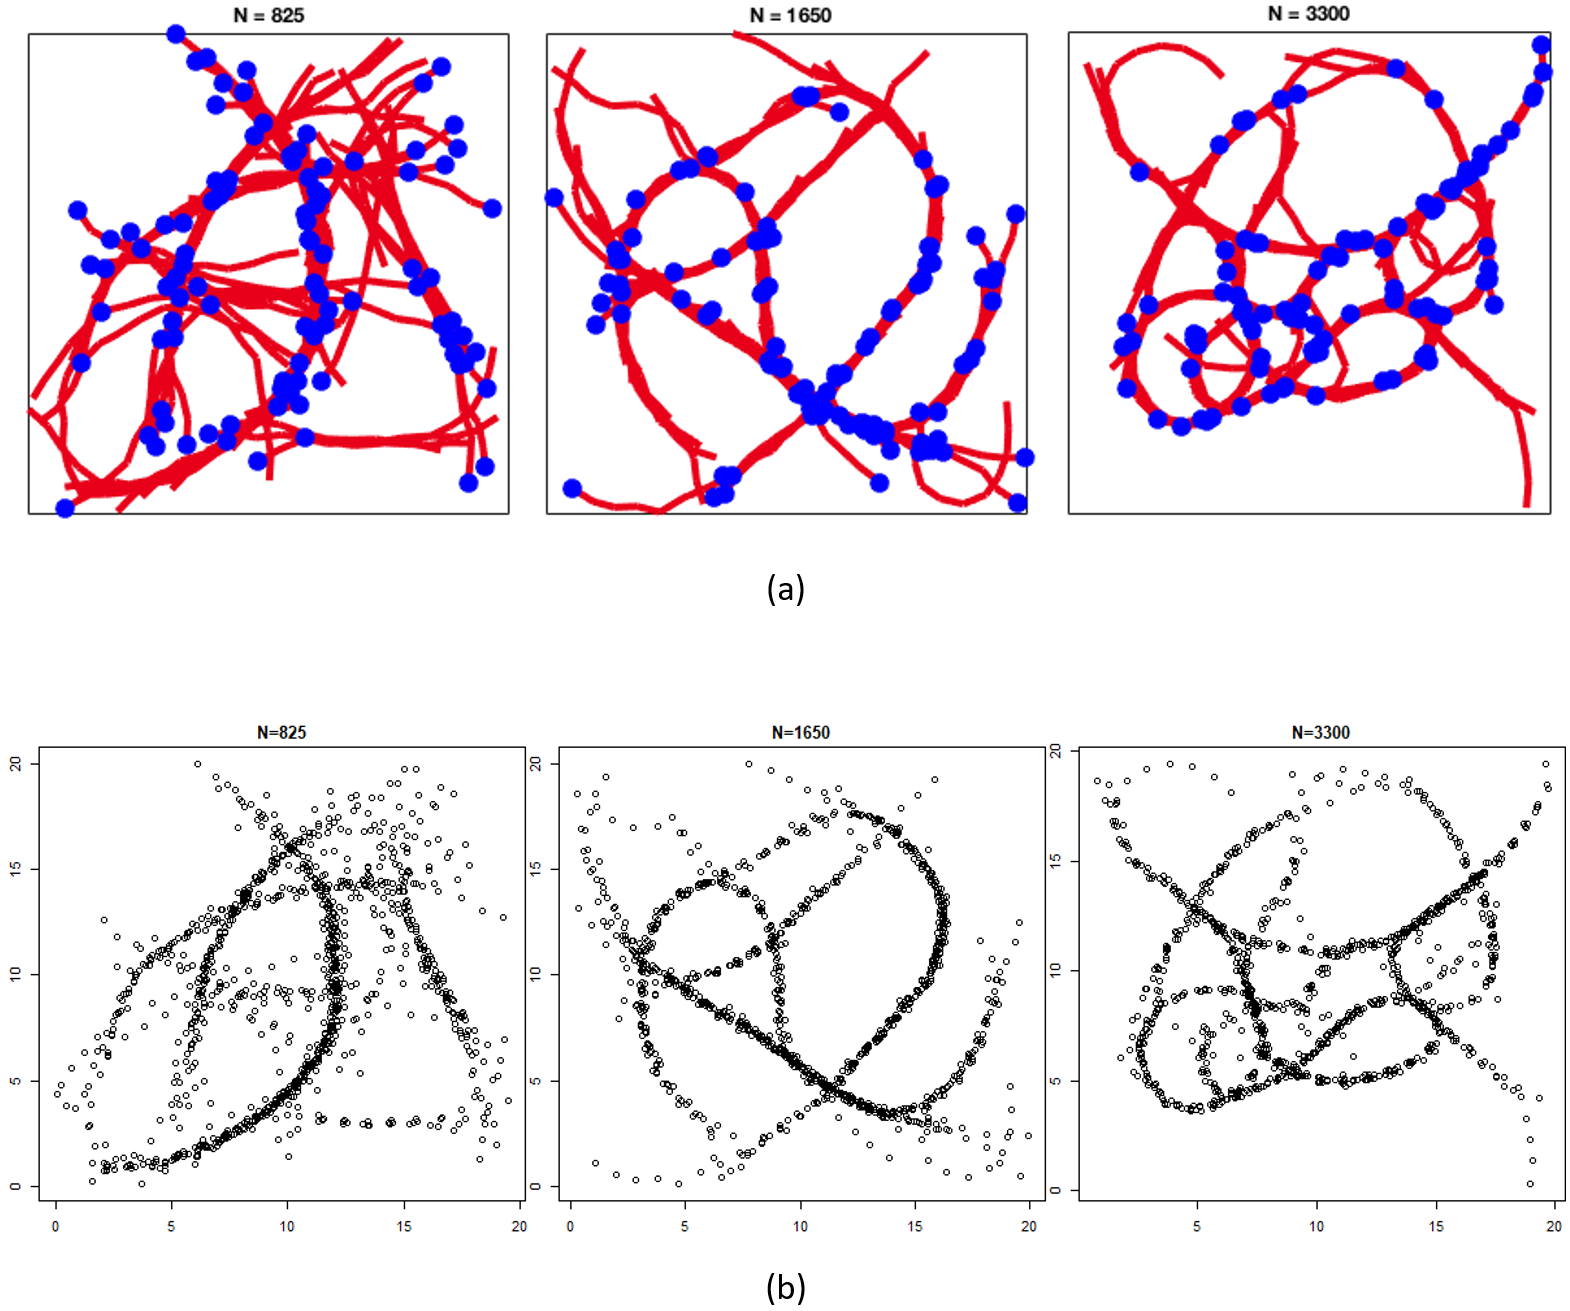
\includegraphics[width=.8\textwidth]{rawdata.png}
	\end{center}
	\caption{Filament networks. Panel (a) shows three filament networks generated by $825$, $1650$ and $3300$ cross-linkers, respectively, in a $\SI{20}{\micro\metre} \times \SI{20}{\micro\metre}$ area. Each network contains $100$ filaments which are represented as red lines. The blue dots are the barbed ends of these filaments. Panel (b) shows the locations of the actin beads that make up the filaments exhibited in Panel (a).}
	\label{fig:rawdata}
\end{figure}

\subsection{Persistence Homology}
In order to build simplicial complexes, we adopt the procedure of forming Vietoris-Rips complexes on each dataset (actin network) by introducing a sequence of $\epsilon$-balls with increasing radius $\epsilon$ centered at each data point (a sampled pixel for the image data or an actin bead for the simulated data). Simplicial complexes are constructed based on intersections of these $\epsilon$-balls and each value of $\epsilon$ corresponds to an unordered group of homological features, which is called a homology group. Considering values of $\epsilon$ as a timeline, we only record when a homological feature appears and disappears. These indexes are called the birth times and death times of the homological features. Moreover, the lifespan (death minus birth) of a homological feature is referred to as the feature's persistence. A set of homological features gives rise to a set of persistence measures. At the end of the procedure, when radius $\epsilon$ is sufficiently large so that the homology group remains unchanged by any further increase to the $\epsilon$, information about a filament network's persistence homology (the set of persistence homology measurements) is summarized in a persistence barcode and/or diagram.

\begin{figure}[H]
	\begin{center}
		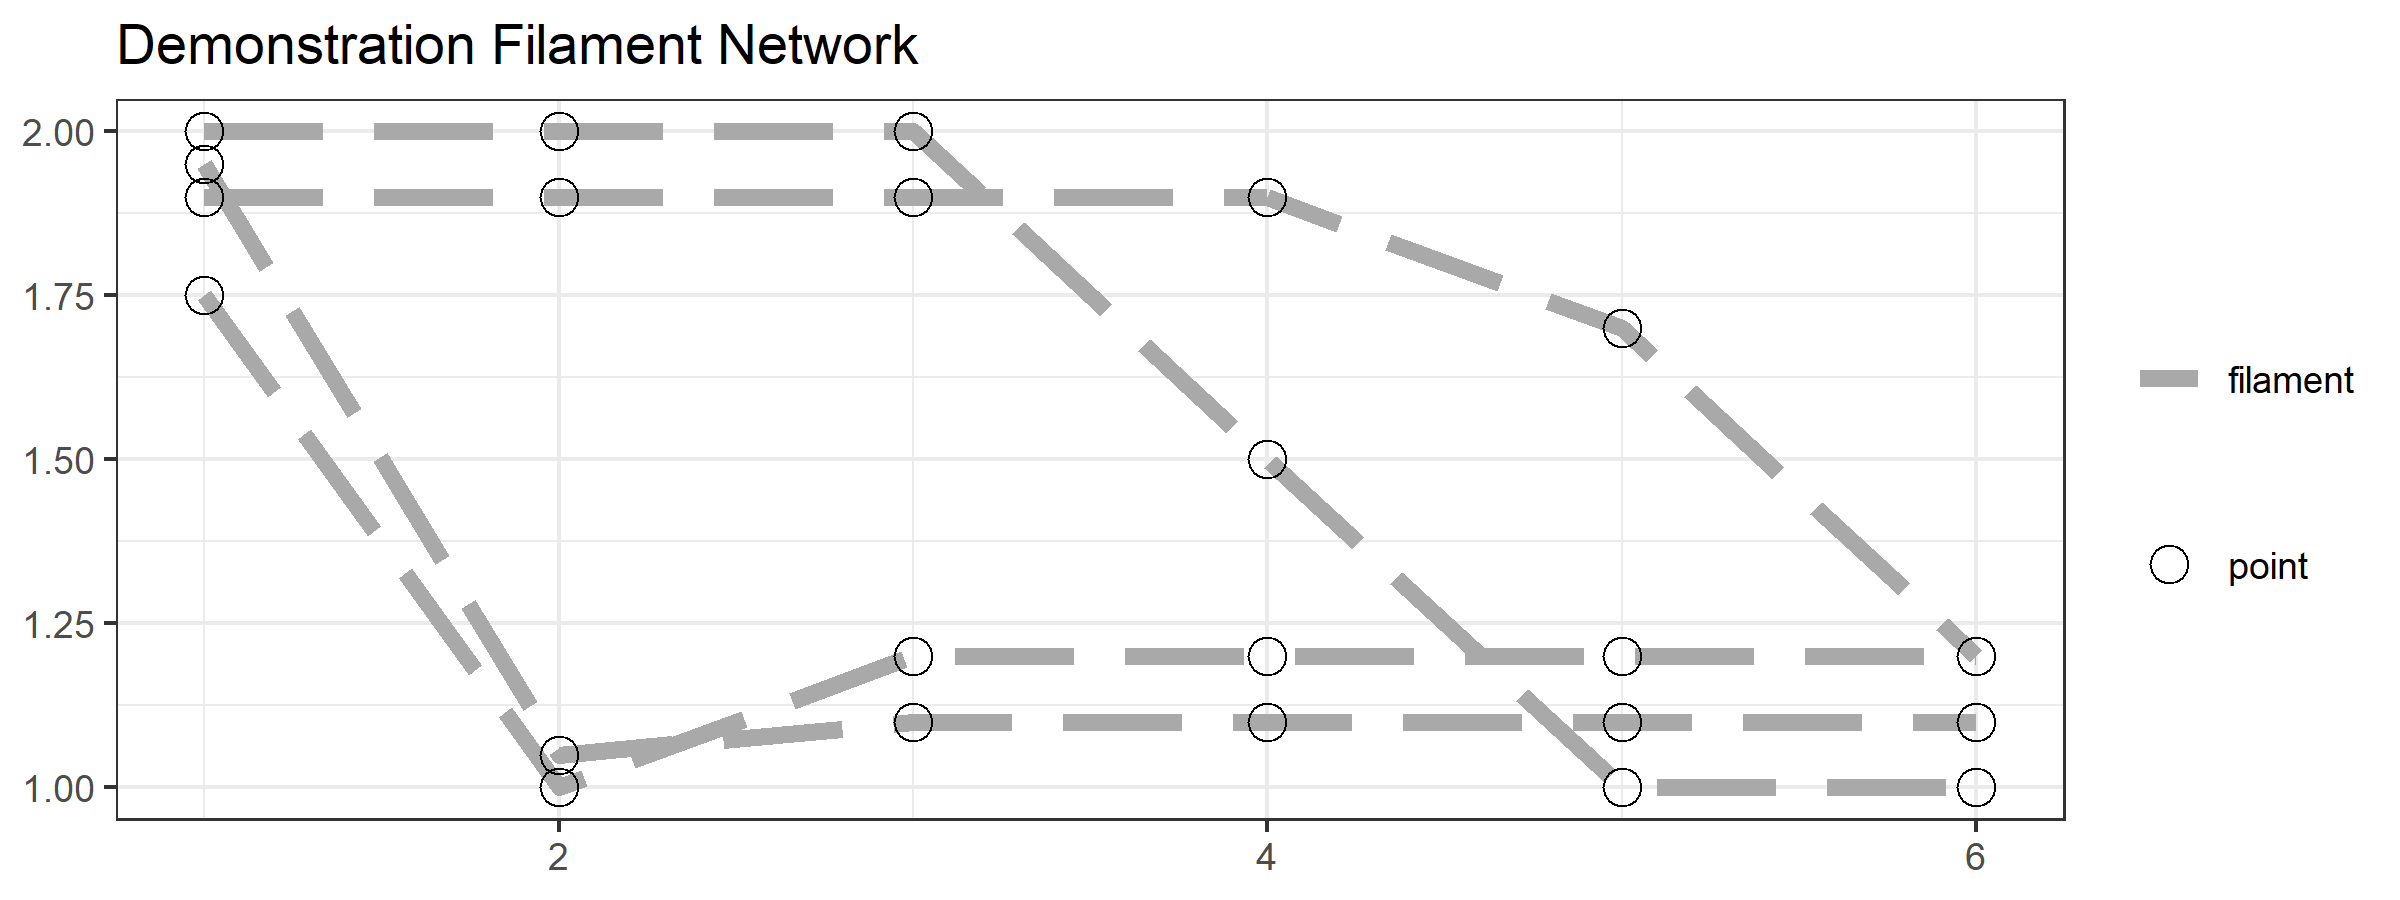
\includegraphics[width=.75\textwidth]{figures/filaments_demo.png}
	\end{center}
	\caption{Demonstration fillament network. This network contains 3 filaments. Points are sampled along the filaments simil, in order to produce a point cloud from which persistence homology can be studied.}
	\label{fig:demoNetwork}
\end{figure}

For clarity, we demonstrate the formation of the persistence on a filament network. We use a simplified filament network which is shown in detail in Figure \ref{fig:demoNetwork}. Figure \ref{fig:persistencediagram} depicts the process of discovering and summarizing the persistence homology of the simple network shown in Figure \ref{fig:demoNetwork}. These illustrations should make clear the connection between filament networks, the Vietoris-Rips Complex and the encoding of the persistence information. 

\begin{figure}[H]
	\begin{center}
		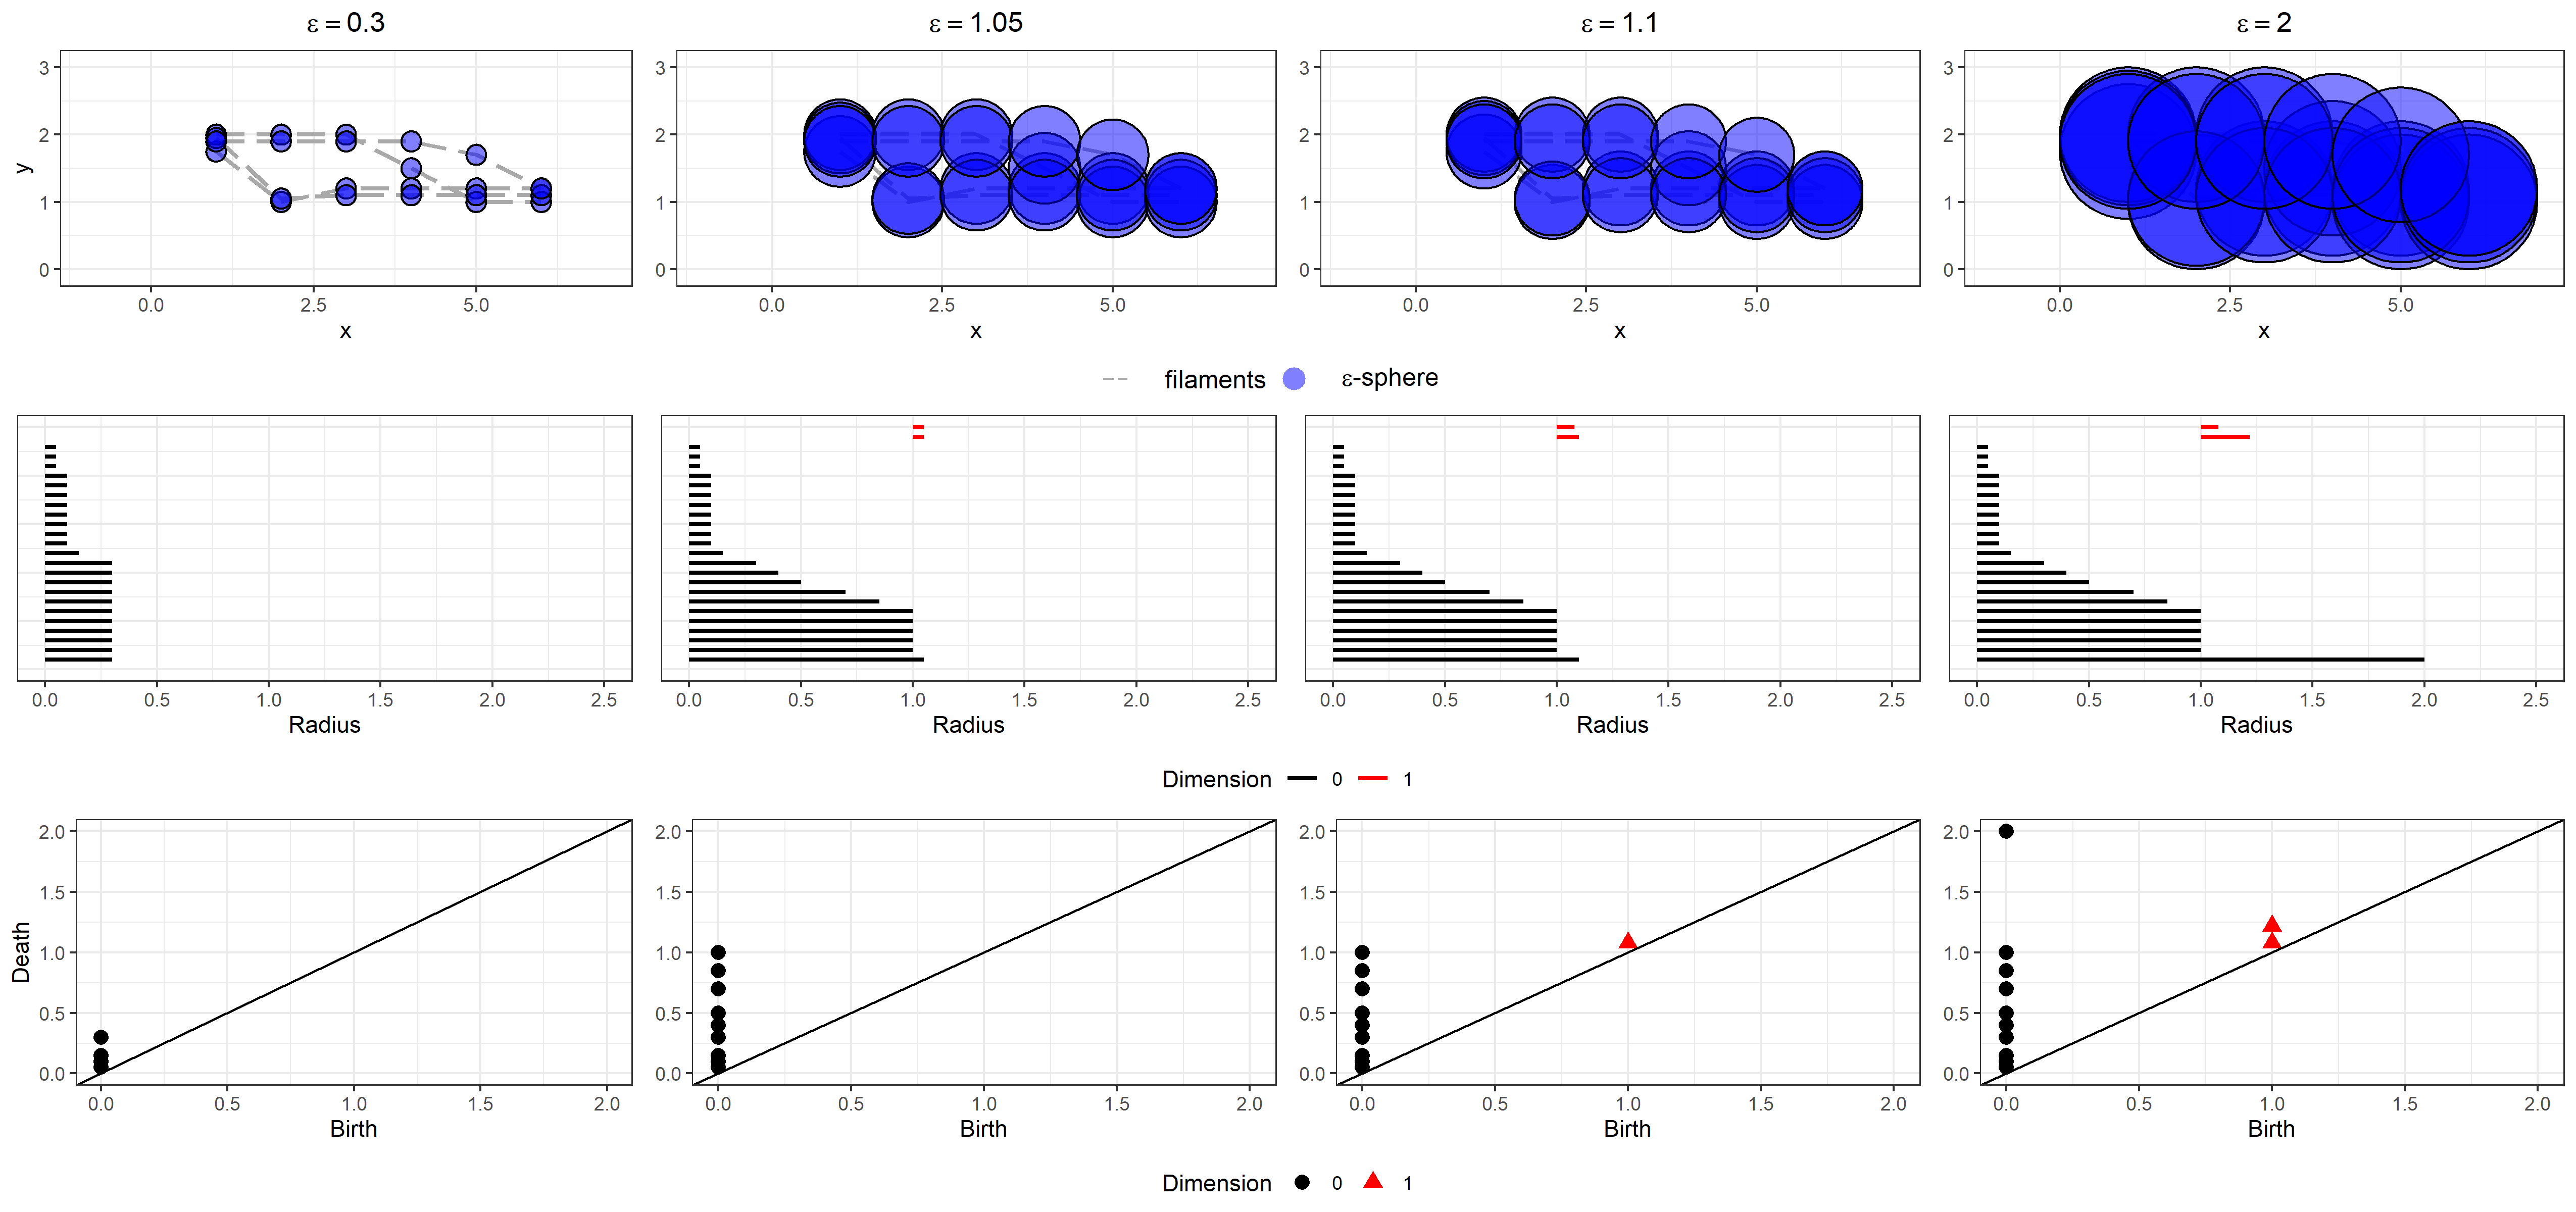
\includegraphics[width=1\textwidth]{figures/filaments_rips.png}
	\end{center}
	\caption{Investigation of the persistence homology of the demonstration filament network in Figure \ref{fig:demoNetwork}. The first row of figures, showes the growing $\epsilon$-spheres about the sampled points of the fillaments. The second row shows the corresponding persistence barcode. The third row shows the corresponding persistence diagram. The columns progress with the algorithm, right-to-left.}
	\label{fig:persistencediagram}
\end{figure}

When $\epsilon=0$, the sampled points of the filament network are each their own connected component. As the $\epsilon$-spheres grow, connecetd components begin to merge. In the first column of Figure \ref{fig:persistencediagram}, when $\epsilon=0.3$, several of the sampled points have already connected. We denote the points which have died (having connected into a larger connected component), by ending their bar in the persistence barcode below. In the third row (of persistence diagrams), we plot a point at 0 (their birth) on the x-axis and at their precise time of death on the y-axis. When $\epsilon\approx1$, two holes form. The holes are evident in the top row, second column, of Figure \ref{fig:persistencediagram}, where one can see a larger and a smaller hole. We begin plotting bars for the holes in the corresponding persistence barcode below. Note that there are not yet reccords (points) for the holes in the persistence diagram. This is because we must know the death time of the holes in order to plot them in the 2-dimensional persistence diagram. 

In the third column of Figure \ref{fig:persistencediagram}, when $\epsilon=1.1$, the smaller hole has closed, and become part of a larger connected component. Now a single point (red triangle) is plotted in the persistence diagram below and the corresponding bar in the persistence barcode is terminated.

As the algorithm progresses, the larger hole eventually dies and its corresponding bar in the final persistence barcode is terminated. A point is also added at the corresponding birth and death in the persistence diagram (a second red triangle appears in the final column, bottom row of Figure \ref{fig:persistencediagram}). The algorithm could continue to $\epsilon=\inf$, but it is evident in this example that no more homological information will be discovered as the spheres continue to grow. We choose to terminate the algorithm at $\epsilon=2$, terminate the final bar in the persistence barcode, and plot a point at (0,2) in the persistence diagram to denote final death time of the connected component which includes all the merged spheres.

Persistence homology indirectly summarizes the hidden shape of the data. In this work, we transcribe the persistence information of each cell to a persistence diagram. Having reccorded the persistence information of the networks, a classifier can be generated either from the distance \cite{marchese2018signal} between persistence diagrams or by alternative vectorizations of the diagrams \cite{adams2017persistence,bubenik2015statistical,maroulas2018stable}. Equipped with persistence diagrams, we will now detail several methods of classification built on the diagrams' homological information.

\section{Methods}\label{sec:methods}
We divide our methods into two subsections. In Subsection \ref{sec:Sub-sampling}, we describe our methods of sub-sampling the simulated and real data. Since the microscopy data and the simulated data live in two distinct spaces, the sub-sampling procedure varies between the two data spaces. Next, in Subsection \ref{sec:classification}, we describe the classifiers used in this work. These vary primarily by whether a vectorization of the persistence diagram is performed for an ML approach, or a distance is calculated between diagrams for a traditional TDA approach. The same classifiers can be applied to both the simulated and the real data.

\subsection{Sub-sampling}\label{sec:Sub-sampling}

\subsubsection{Sub-sampling microscopy data}
The provided microscopy images are extremely large for the computation of persistence homology. Several images are over $1.25\mathrm{e}^6$ pixels (data points). At this time, it is computationaly infeasable to compute persistence diagrams for such images using even a small fraction of the pixels. However, we can efficiently compute the persistence homology of several independent, small sub-samples. Since the intensity of each pixel should be correlated to the probability of the presense of an actin filament in that region of the cell, we can use the pixel intensities as weights on a uniform, random sampler. We take 3 samples, without replacement, of 1000 pixels, where the probability of sampling a pixel is propotionate to its intensity. The coordinates of the sampled pixels then form 3 sub-sampled 1000-point point clouds for which we may calculate a persistence diagram per point cloud.

\subsubsection{Sub-sampling of simulated data}
The simulated data, representing sets of actin beads, included spatial coordinates as well as an index indicating the filament that the beads belonged to. That is, for our networks $\{X_1, X_2... X_{150}\}$, we had 100 filaments in each network $\{F_1, F_2... F_{100}\}$ and each network's sampled points are triples ($x, y$, $f$), where  $x$ and $y$ are the coordinates in the plane and $f$ is the index in the identity map of $F$. 

Using R’s spatial package, each filament was constructed by connecting the ($x$,$y$) bead-coordinates in each filament. A single filament network was then constructed as a multiline object from the corresponding collection of lines formed from the bead-coordinates. These multiline objects were projected onto square grids of $200\times200$ cells. Then, for each network we sampled the multiline object into a grid with the identity function (i.e. the grid cells have value 0 unless a line and grid cell intersect then the value of the grid cell goes to 1). We now had a grid of 4000 cell values taking 0 or 1 for each simulated cell. We filtered these 4000 values to only those of value 1 and used the corresponding planar coordinates to build  our point clouds, simplicial complexes and persistence diagrams. All sub-sampling steps are summarized in Algorithm \ref{alg:resample}. 

\begin{algorithm}[H]\label{alg:resample}
	Let $X_i \in \{X_1...X_{150}\}$ the set of simulated actin networks. \\
    Let $a \in \{A_{i,(x,y,f)}...A_{i,(x,y,f)}\}$ the set of points in $X_i$. $a$ is a pair, $(i, (x,y,f))$, where $i$ is an index to $X_i$, $x$ and $y$ are planar coordinates and $f$ is an index to a filament of $X_i$, $F_{i,f} \in \{F_{i,1}...F_{i,100}\}$, along which $a$ lies. See Panel A of Fig. \ref{fig:resample_algorithm} for a graphical depiction of one $X_i$. For simplicity, we will describe how our algorithm is applied to $X_1$:\\\\
	1. Reconstruct the paths of each $F_{1,f}$ by connecting $A_{1,(x,y,f)}$. See Panel B, Fig. \ref{fig:resample_algorithm}.\\
	2. We project $F_1$ onto a 200x200 square lattice with the same bounds as the given by the data. The cells, $c_{x,y}$ of the lattice take values $\{0,1\}$, where $c_{x,y}=1$ if it is intersected by one of $F_1$ and 0 otherwise. See Panel C of Fig. \ref{fig:resample_algorithm}.\\
	3. Retain only $c_{x,y}$ where $c_{x,y}=1$.\\
	4. Draw 1000 random $c_{x,y}$ without replacement and call these the elements of $R_{1, r}$. Repeat this twice so that $r$ indexes three new samples drawn from $X_1$. The three colors in Panel D of Fig. \ref{fig:resample_algorithm} denote the index $r$.\\
	5. Generate three separate persistence diagrams, $D_{1,r}$, for the new samples $R_{1,r}$. Shown in Panel E of Fig \ref{fig:resample_algorithm}.	\caption{Sub-sampling Algorithm}
\end{algorithm}

\begin{figure}[H]
	\begin{center}
		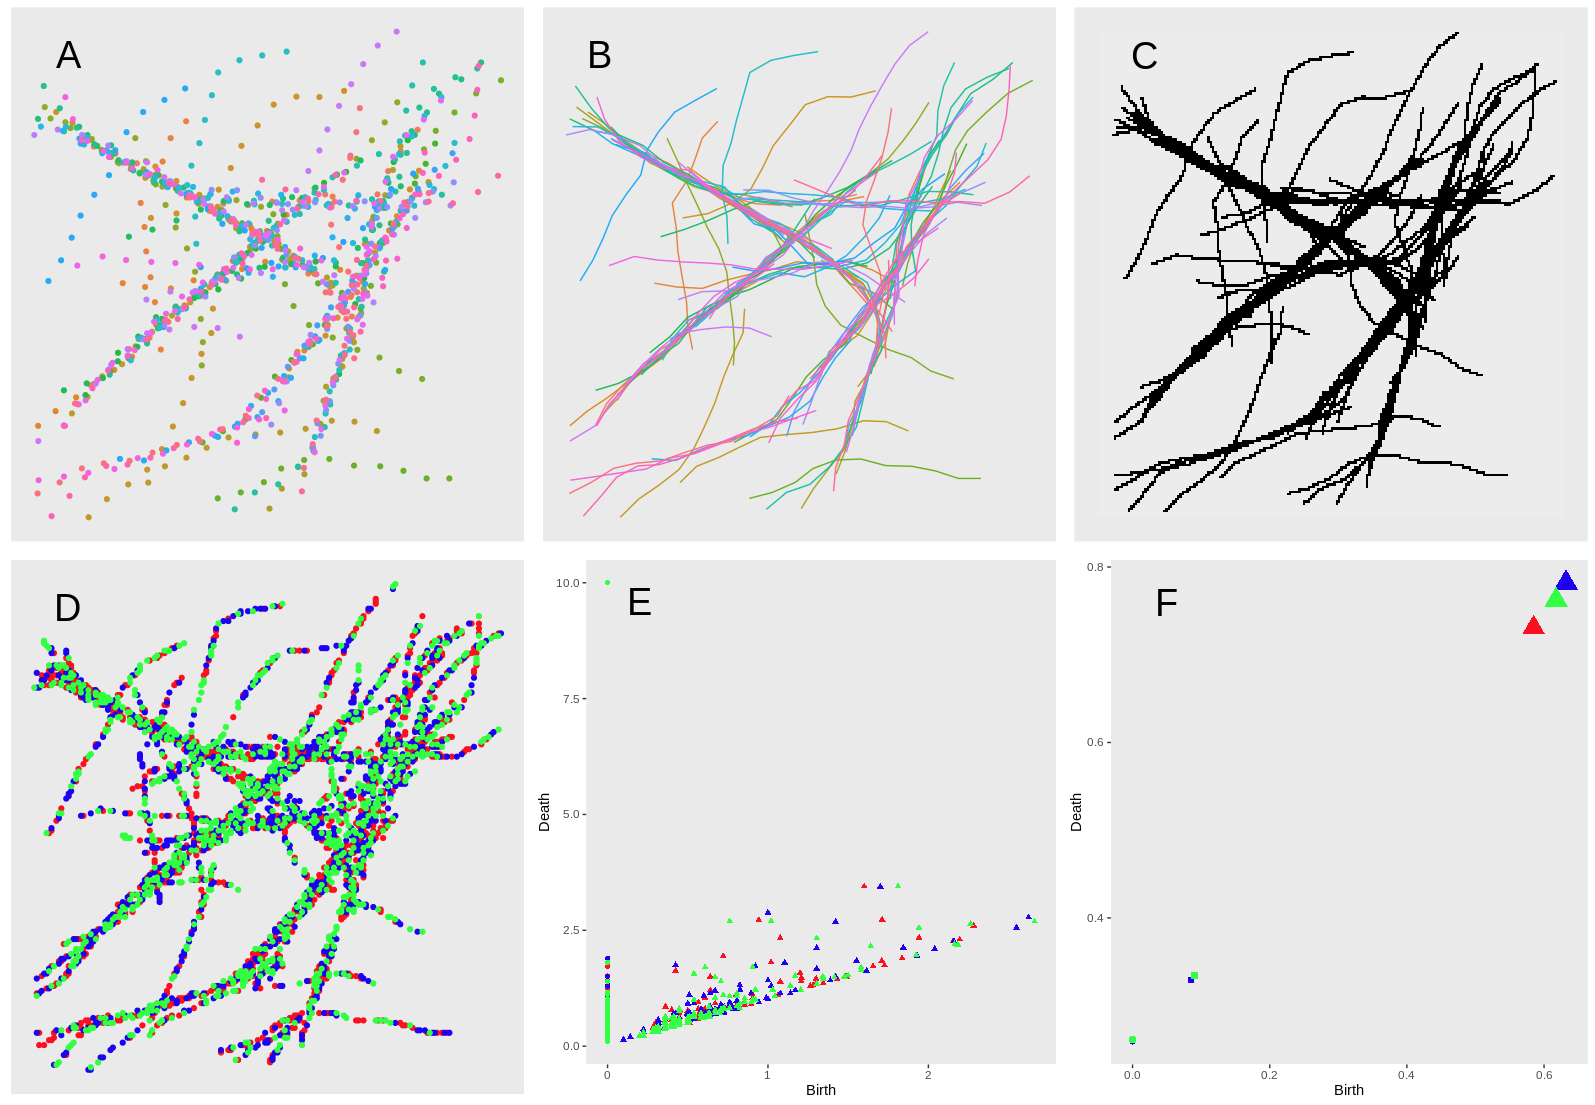
\includegraphics[width=1\textwidth]{figures/resample_algo.png}
	\end{center}
	\caption{Example of one filament construction (B) from the supplied point cloud (A), rasterization (C), sub-sampling (D), construction of persistence diagram (E) and vectorization of persistence diagram (F). The point cloud in (A) was supplied with an index that allowed for the constrution of the filaments in (B); note the coloring. This was projected onto a 200x200 raster (C). The raster was sampled into 3 sets (colored) of 1000 points (D) without replacement and the x,y coordinates are used to generate a VR complex. The persistence diagrams and vectorizations in (E) and (F) are colored the same as (D), to show the variability that arises in the vectorized persistence diagram features when this approach is taken.}
	\label{fig:resample_algorithm}
\end{figure}

As in the microscopy sub-sampling procedure, rather than computing a single Vietoris-Rips complex per network, $1000$ points were randomly sampled from each network $3$ times without replacement. This gives us $3$ sets of $1000$ points per network. This increased the sample size from $150$ to $450$ simulated networks. We computed persistence diagrams for these $450$ networks and used these to construct a classifiers.

\subsection{Classification}\label{sec:classification}


\subsubsection{Persistence vectorization (non-distance based)}
Our key method performs a classification on vectorized features of the persistence diagram. A matrix was generated from the persistence diagrams which had row entries for each diagram and column features with the mean and standard deviation of the persistence diagrams considering only the $0^{th}$ or $1^{th}$ persistence features alone. That is, for each filament network, there is one persistence diagram which corresponds to one row of the vectorized matrix with mean and standard deviation of birth or death times for $0^{th}$, $1^{th}$, or all features. This gives us 12 columnar features. However, the mean and standard deviation of births for $0^{th}$ features are constant 0 and are not considered. Therefore, we are left with 10 entries per vector. This process is identical between the simulated and real data. The vectorization procedure is shown in Algorithm \ref{alg:vectorization}. 

\begin{algorithm}[H]
	We vectorize $D_{1,r}$ from Algorithm \ref{alg:dpcclassifier} by taking the mean $birth$ and mean $death$ of connected components and holes. These data are plotted in Panel F of Figure 3. For $D_{1,r}$ we have 3 row-vectors in the form:
	\begin{center}
	    $v_{1,r}$ =
        $\begin{bmatrix}
            \bar{x}(\mathrm{Death~of~Connected~components})\\
            s(\mathrm{Death~of~Connected~components})\\
            \bar{x}(\mathrm{Birth~of~holes})\\
            s(\mathrm{Birth~of~holes})\\
            \bar{x}(\mathrm{Death~of~holes})\\
            s(\mathrm{Death~of~holes})\\
            \bar{x}(\mathrm{Birth~of~all~features})\\
            s(\mathrm{Birth~of~all~features})\\
            \bar{x}(\mathrm{Death~of~all~features})\\
            s(\mathrm{Death~of~all~features})\\
        \end{bmatrix}$
    \end{center}
	Note: the mean $\bar{x}$ and standard deviation $s$ of the birth of connected components would be $0$ for all vectors, so these are not found in $v_{1,r}$. Repeat for all $X_i$. Our complete matrix of data has a final dimension $450\times10$.\\
	\caption{Vectorization of persistence diagrams}
	\label{alg:vectorization}
\end{algorithm}

With the vectorized data we have the freedom to use any number of commmon classification methods. We present results from implementations of neural networks, random forests, and support vector machines (SVMs).

\subsubsection{Distance-based classifications}

Classifying diagrams in the persistence space, we need a way to quantify the difference between two diagrams. There are two methods commonly used to calculate the distance between persistence diagrams: the Bottleneck and Wasserstein distances \cite{adams2017persistence,bubenik2015statistical,edelsbrunner2010computational,kerber2017geometry,wasserman2018topological} directly from the persistence diagram space. These distances calculate the optimal (minimal) cost in matching the points between two persistence diagrams. They assume infinitely many points of infinite multiplicity on the diagonal (where birth equals death), so that off-carnality points are matched to a point in this artificial set. In addition to the Wasserstein and Bottleneck distances, in this work we adopt a new distance, called $d^c_p$ distance, which is proposed in \cite{marchese2018signal} and has been proved to be stable in \cite{maroulas2018stable}. The cardinality of a persistence diagram may carry important information in applications, especially for those homological features which die very quickly and may be considered as insignificant in Wasserstain distance. However, the $d^c_p$ distance accounts uneven cardinalities between persistence diagrams by assigning a regularization term with the parameter $c$ rather than connecting extra points to the diagonal as is done in the Wasserstein distance. This method allows one to adjust the weight assigned to data that might be considered "topological noise" to fit the particular use case.

\begin{definition}{1}
Let $D_X$ and $D_Y$ be two persistence diagrams with cardinalities $n$ and $m$ respectively such that $n \leq m$ and denote $D_x=\{ x_1,...,x_n \}$, $D_y=\{ y_1,...,y_m \}$. Let $c>0$ and $1\leq p <\infty$ be fixed parameters. The $d^c_p$ distance between two persistence diagrams $D_x$ and $D_y$ is
\begin{align}
    d^c_p(D_x,D_y)= \left( \frac{1}{m} \left( \min_{\pi \in \Pi_m} \sum^n_{l=1} min(c,||x_l-y_{\pi(l)}||_\infty)^p+c^P|m-n|  \right) \right)^{\frac{1}{p}},
    \label{eq:dpcdistance}
\end{align}
where $\Pi_m$ is the set of permutations of $(1,...,m)$. If $m<n$, define $d^c_p(D_x,D_y):=d^c_p(D_y,D_x)$.
\end{definition}

The $d^c_p$ distance not only calculates the distance of points in two persistence diagrams without the simulated points on the diagonal, it also adds a penalty term on the difference in cardinalities of the two sets of points. The parameter $c$ in eq. (\ref{eq:dpcdistance}) is a constant that controls the weight of penalization to be added in the $d^c_p$ distance. Larger values of $c$ will yield a larger penalization. The parameter $p$ is typically chosen as $2$ since this corresponds to the Euclidean distance. We tend to evaluate $c$ between $0$ and $1$ as these have been empirically found to be appropriate options in real-world applications \cite{maroulas2018stable}.

Since persistence diagrams can summarize the homological features of multiple dimensions in one diagram, such as in the last panel of Fig. \ref{fig:persistencediagram}, the persistence diagram contains both $0$-dim features(connected components) with cardinality $5$ and $1$-dim features(holes) with cardinality $1$. We can further define the $d^c_p$ distance of a certain dimensional feature between a persistence diagram and a group of persistence diagrams.

\begin{definition}{2}
Denote $\D$ as a collection of persistence diagrams in the same class. For a specific $\beta$-dim homological feature, $\beta=0,1,2,...$, the $d^c_p$ distance between a persistence diagram $D_x$ and the set of persistence diagrams $\D$ is
\begin{align}
    d_\beta (D_x,\D)=\frac{1}{|\D|}\sum_{D \in \D} d^c_p(D_x,D),
    \label{dpcsets}
\end{align}
where $|\D|$ represents the size of class $\D$.
\end{definition}

With all preparations above complete, we can build the $d^c_p$-based network classifier. For $K$ classes of filament networks, every network in a class is generated under a unique set of constraints. Therefore, we have $K$ sets of persistence diagrams, where each set corresponds to a class of network generated under unique constraints. Given a new filament network with its persistence diagram $D'$, our goal is to classify under which constraints the network was most likely generated, i.e. to which class $k$ it most likely belongs. We can estimate this membership by calculating the distance between $D'$ and each class of persistence diagrams. We then assign the new network to the class with the smallest distance. Additionally, we parameterize the relative weights for different dimensions of homological features in the calculation of the distance and force the weights' sum to $1$. The classifier is summarized in Algorithm \ref{alg:dpcclassifier}.

\begin{algorithm}[!htbp]
	Let $B$ is highest dimension of homological features under consideration.\\ 1. Take the training set $T_1, T_2,..., T_K$ from each class of diagrams $\D_1,\D_2,...,\D_K$, \\
	2. For a new network with its corresponding persistence diagram $D'$, compute
	\begin{align}
	    d(D',T_k)=\sum^B_{\beta=0} w_\beta d_\beta (D',T_k),
	\end{align}
	\ \ \  where $\sum^B_{\beta=0}w_\beta=1$, and $w_\beta$ determine how much $\beta$-dim homological feature is considered,\\
	3. Assign $D'$ a class label $c'$ such that,
	\begin{align}
	    c'=\argminA_{1\leq k \leq K} d(D',T_k),
	\end{align}
	\caption{$d^c_p$-based network classifier}
	\label{alg:dpcclassifier}
\end{algorithm}


\subsection{Prediction}
The sub-sampling procedure introduces one idiosyncrasy, which is an ambiguity of how to utilize multiple predictions per network. For classifiers using sub-sampled data, predictions were made for each of the test-fold sub-sampled networks $R_{i,\chi}$. These predictions were considered as votes and the majority label was taken as the final prediction for $X_{\chi}$. This returns us to a state of one prediction per test-fold network.

\section{Results}\label{sec:results}
The cross-validated ($k=10$) classification of the simulated networks was performed with many common, competing methods. The top performer was a support vector machine (SVM), trained on the sub-sampled and topologically transformed data. The next best performance was achieved by the $d^c_p$-based classifier. We also provide the accuracy rates of several other classifiers tested in Table \ref{tab:accuracyrate}.

\begin{table}[H]
	\begin{center}
		\begin{tabular}{c|c}
			\hline
			\textbf{classifier} & \textbf{mean accuracy} \\
			\hline
			SVM, re-sampled & 94\%  \\
			\hline
			$d^c_p$-based & 89\%  \\
			\hline
			Wasserstein-based, re-sampled & 87\%  \\
			\hline
			Wasserstein-based & 83\%  \\
			\hline
			Bayes Factor \cite{maroulas2019bayesian} & 83\%  \\
			\hline
			SVM PI \cite{adams2017persistence} & 75\%  \\
			\hline
			Neural Net PI & 71\%  \\
			\hline
			SVM Raster & 65\%  \\
			\hline
			Random Forest Raster & 55\%  \\
			\hline
		\end{tabular}
		\caption{Cross-validated accuracy rate of classifiers on simulated actin networks.}\label{tab:accuracyrate}
	\end{center}
\end{table}

Our findings show that sub-sampling of data can produce a more reliable filament network classifier even when data are mapped to a topological space and summarized in persistence diagrams. The $d^c_p$-based classifier performed much better than Wasserstein-based classifier. Since, our re-sampled and vectorized persistence diagram far outperformed all other classifiers, we proceeded to test this method on the microscopy data.

We perform classification of MMs and WTs using our top classifier, the re-sampled SVM. The data are provided as tifs from 22 MM and 20 WT cells ($n=42$). We find a cross-validated ($k=5$) accuracy of approximatley 83\%. We used fewer folds in testing accuracy on the microscopy data, only because of the relatively samll sample size.

\section{Discussion}\label{sec:discussion}
In this work, we propose a machine learning approach to classify filament networks generated with varied cross-linker density. Our method leverages the topology of the actin networks through a topological transformation. Our exploratory work is the first time filament networks have been studied by homological classification. This work should be useful in the course of research on cytoplasmic streaming. This tool provides biologists a method of disentangling the interaction of myosin motor proteins, the actin network, and streaming, i.e. by imaging the actin structure and clustering cells based on their actin network topology, the researcher should be able to fix a network structure while varying parameters specific to myosin.

The microscopy experiment differs from the simulated experiment in that our simulated experiment involved the direct manipulation of the actin network through changes in cross-linker abundance. The groups in the microscopy experimetn differ in by a far less direct manipulation. Whereas cross-linking is fundamental to the structure of the actin network, the linkage betweeen a single type of mysoin motor and resulting actin networks is more complex and likely modulated by several interacting factors. The simulated actin networks were critical to the development of our new tool, both in their clarity and in that they allowed us to benchmark algorithms without overfitting to our small sample of microscopy data.

Interpretation of these results is complicated by our uncertainty of the true, cumulative impact of a myosin knockout on the actin network. While the accuracy of our method on real data is significantly lower than found in the analysis of the simulated data, this could easily be explained by the single motor protein knockout having a relatively minor impact on actin organization when compared with up or down regualtion of cross-linkers. Out of curiosity, we conducted a small survey (\textit{n}=6), wherein we asked respondents who were familiar with the experiment to sepparate the cells into two classes. We found that respondents had an average accuracy of 63\%, with a minimum accuracy of random chance and a maximum accuracy of 75\%. Since our algorithm is more effective than manual classification by an expert, we are left to conclude that there is likely a weak relationship between this mysoin knockout and actin network structure, and our classification algorithm is likely running into the ceiling of discernible difference in classes.

\subsection{Conclusion}
In sum, we successfully classified simulated actin filament networks generated under three different initial conditions with very high accuracy. We combined a machine learning framework with TDA for our classification. We compared this method with several distance-based classifiers. Our most successful method uses a sub-sampling technique, a vectorization of the persistence diagram, an SVM as the classifier and a voting mechanism for the final predictions. We then showed an application of our method to real confocal microscopic data. Our methods were built on the foundation of topological homology by encoding geometric features hidden in the data into the topological features and summarizing those into persistence diagrams.

In future work, we hope that this method will reveal key factors in the filament network organizing process and provide biologists with opportunities to study the interaction of motor proteins, actin networks and cytoplasmic streaming. We demonstrate that it is simple to bridge our method between simulations and real images, laying the groundwork for additional work comparing outcomes of simulations to real experiments.

\clearpage	
\bibliographystyle{plain}
\bibliography{bibliography}


\end{document}
